\epigraph{``Curious that we spend more time congratulating people who have succeeded than encouraging people who have not."}{Neil deGrasse Tyson}

\section{Open Source Software}
As mentioned previously, and to the author's knowledge, there is no open source software currently available that can numerically simulate the dynamics of the atmosphere. But, what is open source software, what are its advantages, and why is it important?

\begin{definition}
Open Source Software is software with source code that anyone can inspect, modify, and enhance. 
\end{definition}

Source code is the code that computer programmers use to modify, and change how a piece of software functions\cite{what_oss}. Programmers with access to the source code can improve that program by adding features to it, fixing bugs, or by improving the documentation of the surrounding source code. 

According to Tom Macaulay\cite{advantages}, the open source development of software has a number of advantages over the traditional development of proprietary software, including but not limited to:

\begin{itemize}
    \item Lower costs.
    \item Extensive customisation.
    \item Higher quality software.
    \item Greater security.
    \item Regular updates.
    \item Quick fixes.
\end{itemize}

If an atmospheric dynamics simulator became available to the open source community, it could lead to a low cost, and high quality simulator ultimately being produced. If such an event occurs, it could, theoretically, vastly enhance existing weather predicting software, and could lead to a further dramatic decline in deaths from weather related phenomena. This project is an attempt to kick start such a future.

Everything related to this project, from the source code of the simulator to this very paper, can be accessed at the organisation known as `AMSIMP' on the open source platform known as GitHub. This can be accessed at \url{https://github.com/amsimp}. 

\begin{figure}[H]
    \centering
    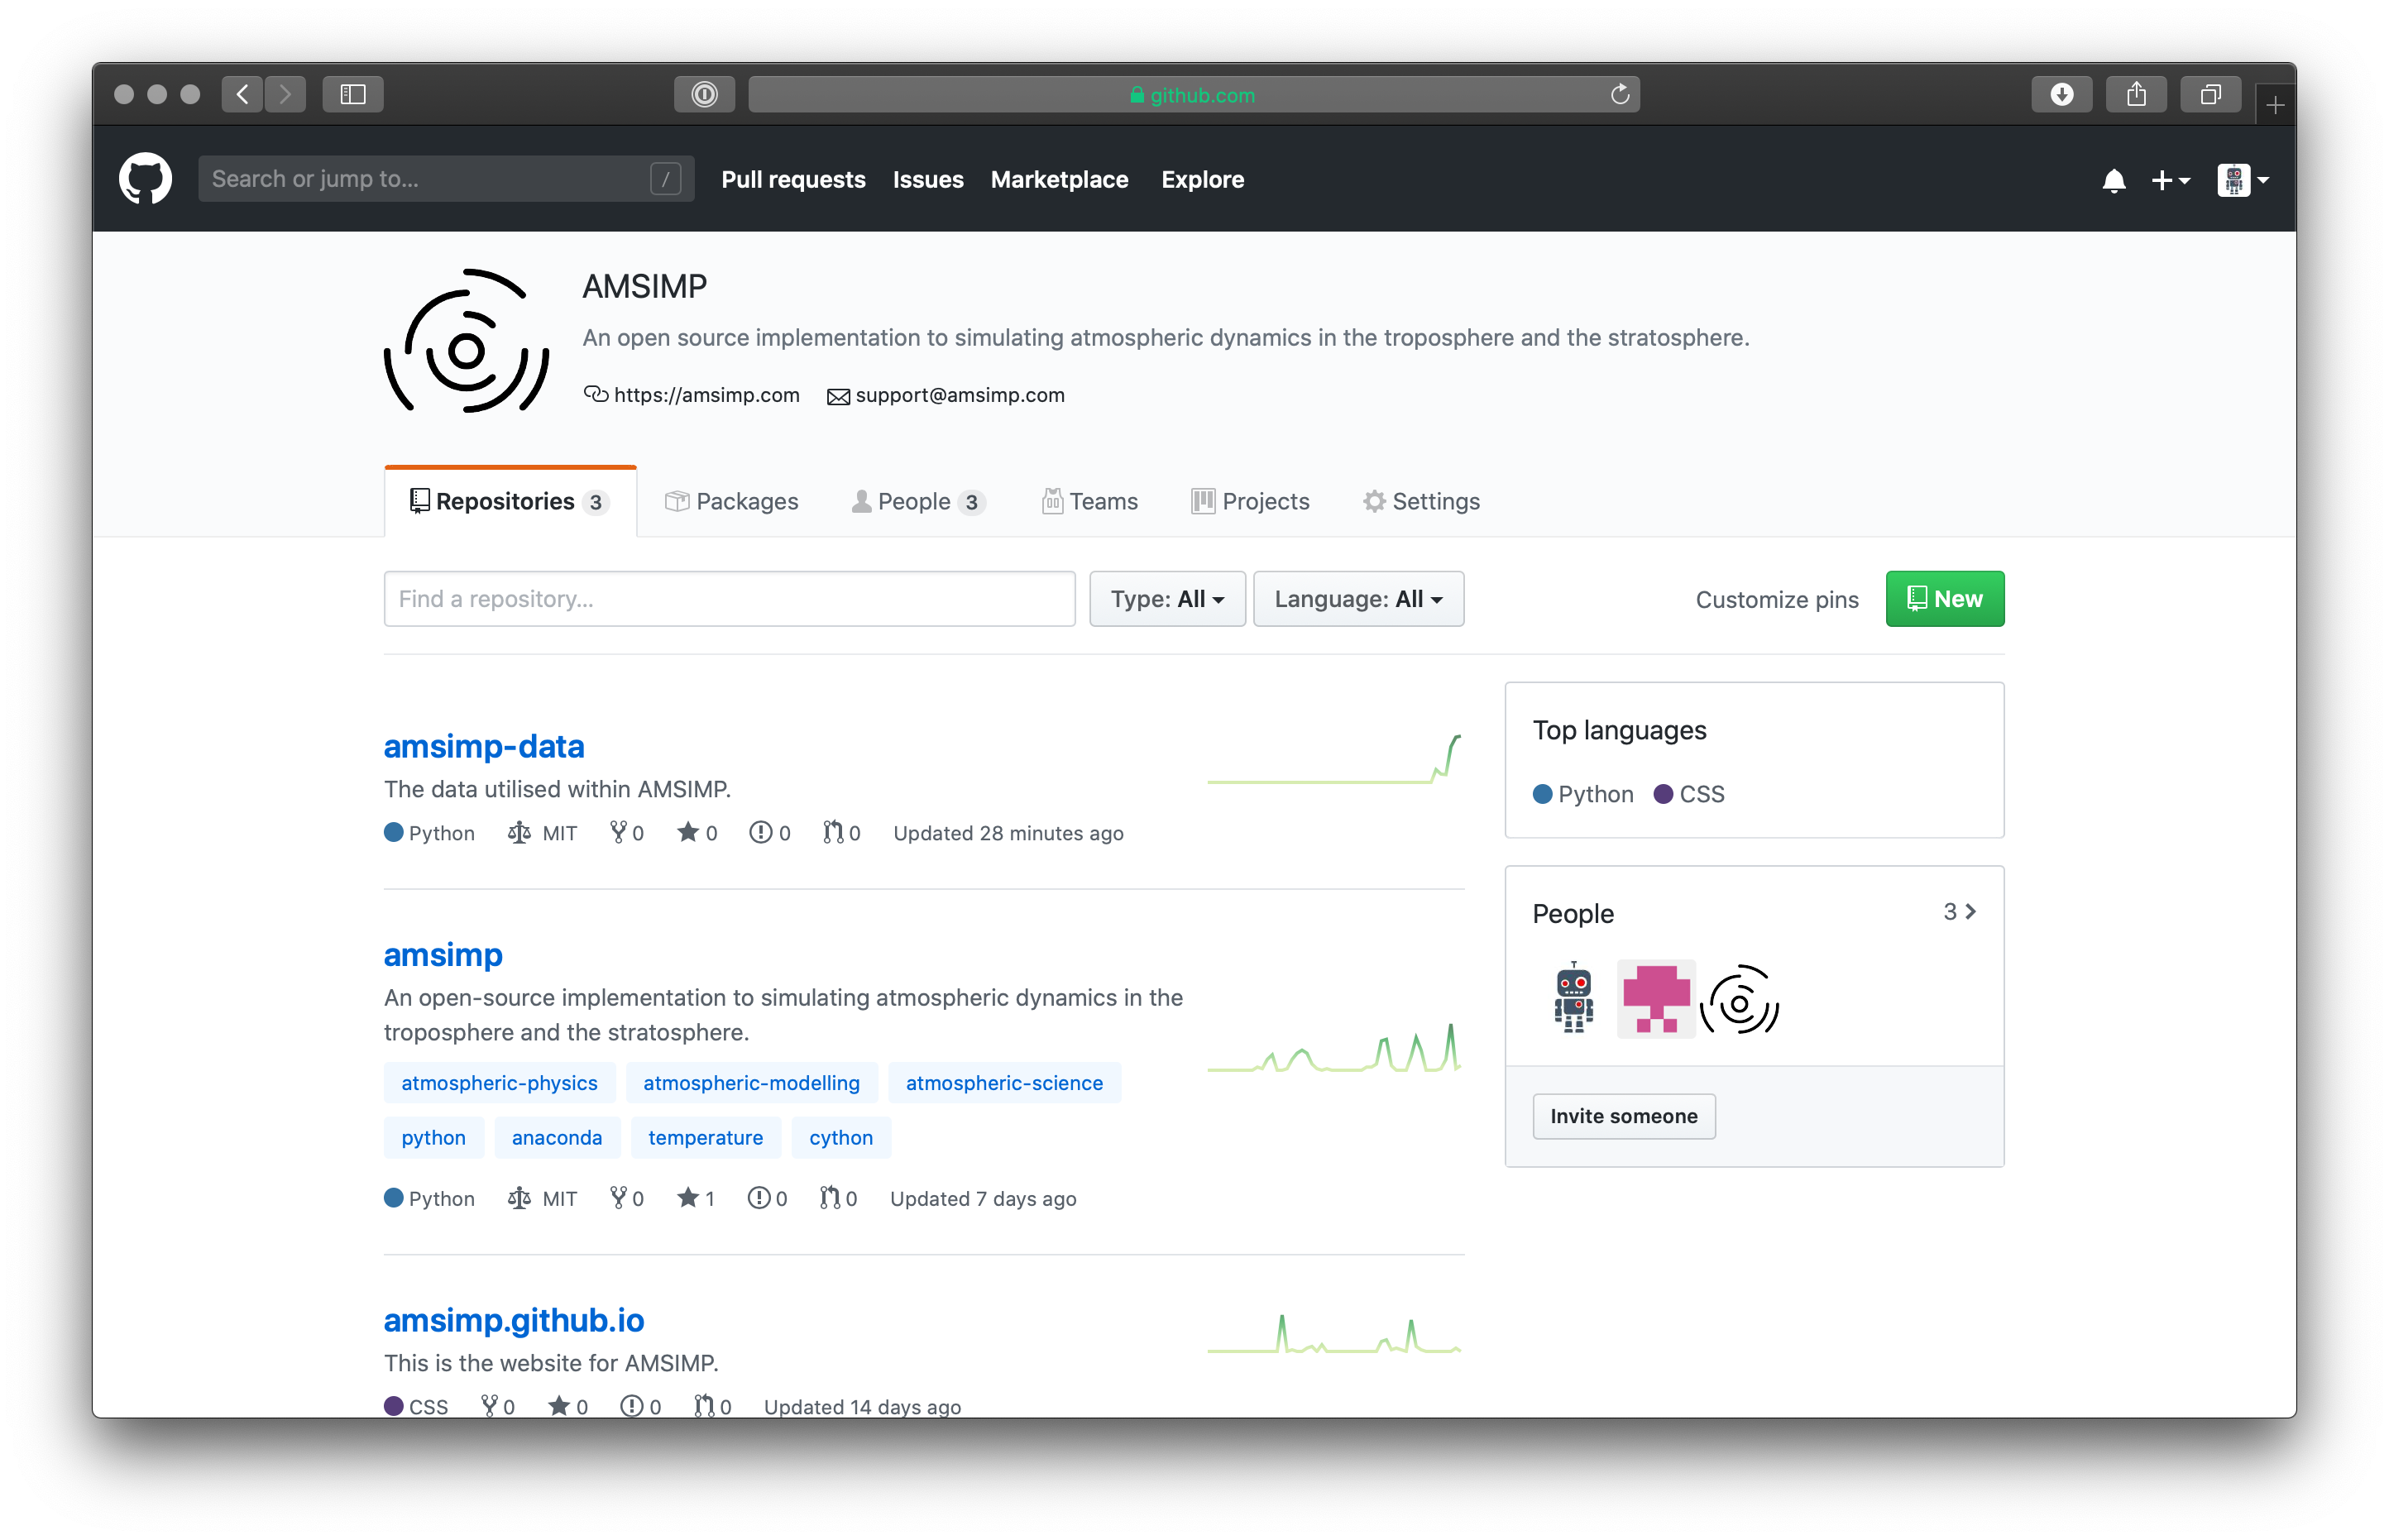
\includegraphics[width=.8\linewidth]{Images/github}
    \caption{A screenshot of the AMSIMP organisation, hosted by the open source platform known as GitHub.}
    \label{github}
\end{figure}

\section{Language Selection}
\subsection{Initial Language Selection}
The most crucial element of this project was choosing an appropriate programming language for the task. During the initial consideration period, I analysed two different programming languages: JavaScript, and Python\cite{python}. 

Initially, I considered the programming language, JavaScript with a run-time environment known as Node.js (Node.js executes code outside of a browser), for two reasons primarily:

\begin{itemize}
    \item JavaScript excels at data visualisation.
    \item Node.js is extremely well suited for memory intensive activities.
\end{itemize}

In line with the expectation of using this programming language, Miss Abbott, and I attended the Dublin Node.js Meetup on the 28th of February. I did this in order to gain an understanding of what Node.js is used for, and what would be the best way one would go about using it. 

In the end, however, I ultimately chose Python for the task due to a number of shortcomings on the part of JavaScript (Node.js), and advantages on the part of Python. Firstly, JavaScript just doesn’t have the same enormous suite of scientific packages and inbuilt functionality that Python does. Using JavaScript, therefore, would waste valuable development time, and ultimately would be entirely inefficient.

Secondly, Python already has an extensive ecosystem with how-to’s available for almost any scientific task you would ever want to do. For JavaScript, this is simply not the case.\cite{javascript_vs_python}

\subsection{Switching to Cython}
During the continued development of the software over the summer months, I discovered a rather severe bottleneck as a result of my choice of programming language: the execution time performance. The culprit behind this bottleneck was a result of Python's dynamically typed nature. Generally, you can classify programming languages into two categories: dynamically typed languages and statically typed languages. 

\begin{definition}
A dynamically typed language is one in which the type of the variable is not known at compile time, and generally, you can define a variable as an integer type at the start of the program for example and later redefine it as a string type. 
\end{definition}

On the other hand, a statically typed language is a language where the type of variable is known at compile time, and during the execution of the program, the variable type must remain constant. 

\hfill

\begin{figure}[H]
    \centering
    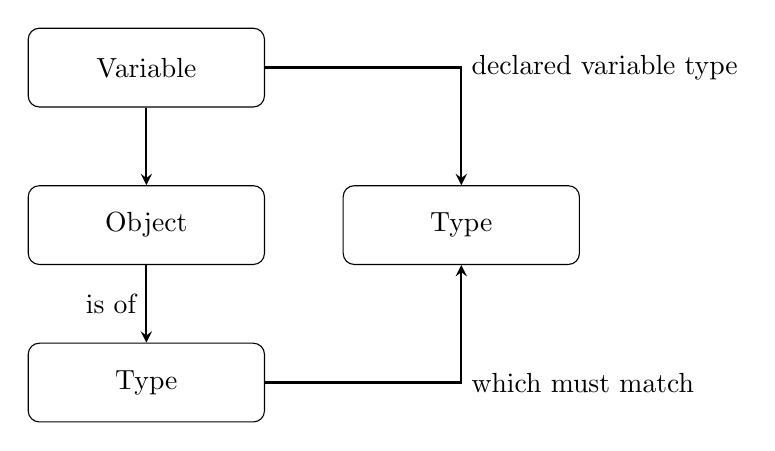
\begin{tikzpicture}[node distance=2cm]
        \tikzstyle{startstop} = [rectangle, rounded corners, minimum width=3cm, minimum height=1cm,text centered, draw=black]
        \tikzstyle{arrow} = [thick,->,>=stealth]
        
        \node (start) [startstop] {Variable};
        \node (obj) [startstop, below of=start] {Object};
        \node (type1) [startstop, right of=obj, xshift=2cm] {Type};
        \node (type2) [startstop, below of=obj] {Type};
        
        \draw [arrow] (start) -- (obj);
        \draw [arrow] (start) -| node[anchor=west] {declared variable type} (type1);
        \draw [arrow] (obj) -- node[anchor=east] {is of} (type2);
        \draw [arrow] (type2) -| node[anchor=west] {which must match} (type1);
    \end{tikzpicture}
    \caption{How statically typed languages handle variables.}
\end{figure}

A statically typed language is particularly useful for software with a large number of loops, or repetitive calculations contained within them. During a loop, a dynamically typed language will continuously check the type of variable after each loop, even if it has done so in previous loops. In a small number of loops, this has a negligible impact on the execution time; however, in a large enough quantity, this has a cumulative effect, significantly stifling the execution time performance. Generally, a piece of software written in a statically typed language will execute a lot faster; this fact will be demonstrated in chapter \ref{6}. The reason behind picking Cython over other statically typed languages, such as C, is that Cython retains all the benefits of Python, with its extensive scientific package library and its simple syntax, while gaining the performance benefits of a statically typed language.

